\documentclass[11pt,a4paper]{article}
\usepackage[margin=24mm]{geometry}
\usepackage[T1]{fontenc}
\usepackage[utf8]{inputenc}
\usepackage{lmodern,amsmath,amssymb,booktabs,graphicx}
\usepackage[colorlinks=true,allcolors=blue]{hyperref}
\newcommand{\E}{\mathbb E}
\newcommand{\Var}{\operatorname{Var}}
\newcommand{\Cov}{\operatorname{Cov}}
\newcommand{\Li}{\operatorname{Li}}
\setlength{\emergencystretch}{2em}
\title{Partial ports and crossing fluctuations in the\\three-dimensional Lorentz mirror model}
\author{JJIN HANZHE}
\date{Version 1.0.0 \quad 3 November 2026}
\begin{document}
\maketitle
\begin{abstract}
Deterministic trajectories in random mirror environments produce fluctuations
between environments. We study their dependence on which boundary ports are
counted. Pure retroreflection on part of a face admits an exact
environment-by-environment reduction to selected connections in a fully open
reference system. Applying established multiterminal diffusive counting theory
gives a conditional variance-to-mean ratio \(1-J/M\), determined by a Laplace
problem. For \(m\) stripes occupying fraction \(p\) of a face, Fourier
evaluation gives
\(1-p/3-[\zeta(3)-\Re\Li_3(e^{2\pi ip})]/(4\pi^3mp)\), up to exponentially
small terms. Two mirror rules and sizes up to \(L=256\) support the half-open
predictions within the reported statistical errors and extrapolation spread.
The two prescribed extrapolations differ by approximately \(0.3\)--\(0.7\%\).
Earlier tests reject \(2/3\) for the retroreflecting count, while its reconstructed
full-face count is consistent with that benchmark. Exploratory quarter-open
layouts lie about \(0.5\%\) high; independent third-cumulant estimates lie on
opposite sides of the saddle value. These discrepancies remain unresolved.
Our contribution concerns this specific reduction, three-dimensional geometry
and numerical tests; partial-boundary counting in loop models and the general
multiterminal framework have precedents.
\end{abstract}
\noindent\textbf{Status: not peer reviewed.}
AI systems performed design, simulation, analysis, derivation and writing under
the author's directional guidance: Opus 5.5 proposed the initial plan and
GPT-6 Astra (max) performed the later work (names supplied by the author).
No external human expert review has taken place. See the README disclosure.

\section{Introduction}
The Lorentz mirror model separates deterministic propagation from random
environment selection. Paired ports prescribe a unique outgoing direction
for each incoming ray. Statistics concern different environments, despite the
absence of dynamical randomness in any one of them. Deterministic lattice
transport and macroscopic diffusion have substantial precedents
\cite{Ruijgrok,Chiffaudel}. Lefevere and Tasaki discuss a \(2/3\)
mean--variance relation and higher crossing cumulants \cite{LT}.
Loop models with crossings provide a related counting-field description
\cite{NSSO}.

The theoretical setting includes Goldstone phases of intersecting loops
\cite{Goldstone}, oriented three-dimensional loops \cite{Nahum2011,Nahum3D},
and unoriented loops with a real-projective description \cite{Serna}.
These results motivate a smooth candidate theory; they do not prove its
complete applicability to both six-valent rules used here.

Diffusive-conductor counting statistics are established
\cite{Beenakker,Nagaev,Blanter,LLY,Nazarov}. Multiterminal noise and full
counting statistics were developed by Sukhorukov--Loss and Nazarov--Bagrets
\cite{SL,SLlong,NB}. Related structures occur in stochastic diffusive systems
\cite{DDR,Bodineau,MFT}. Akkermans and coauthors extend two-reservoir counting
to arbitrary higher-dimensional domains within macroscopic fluctuation theory,
with macroscopic contacts and a stationary saddle \cite{ABDS}.
Here the random object is a quenched environment rather than a
time-integrated stochastic current.

Partial-boundary counting also has a direct loop-model precedent.
Morin-Duchesne and Jacobsen weight connections between a chosen boundary
segment and its complement in a two-dimensional dense-loop model \cite{Morin}.
That geometry and count differ from the present left-face-to-right-subset
observable. Gu, Schaeffer and Hao study fixed-aperture routing and suppression
of nearby transmitting channels in a three-dimensional oriented K-lattice
\cite{Gu}. Boundary spatial correlations are therefore not a new general
observation of this work.

Within the literature we searched, the contribution here is the specific
pure-retroreflection reduction, its three-dimensional stripe evaluation and
quantitative tests. We assert neither a new general counting framework nor
a new universality class. Classical representations of quantum localization
\cite{GLR,Beamond,Ortuno} do not in general equate the fluctuations of the two
problems, as emphasized by Cardy \cite{Cardy}.

\section{Model and observables}
Each cubic-lattice vertex independently receives a uniform perfect matching
of its six ports. The standard rule permits all 15 matchings; the orthogonal
rule permits the eight without an opposite-port pair. Transport is along
the open \(x\) direction; transverse directions are periodic.

Let \(L_{\rm t}\) denote the full left terminal, distinct from side length
\(L\). The right face is partitioned into counted ports \(A\) and complement
\(W\). Write \(C=n_{L_{\rm t}A}\), and let \(N\) count all left-to-right paths
with the entire face open. Cumulants refer to independent environments:
\[
v=\kappa_2(C)/\kappa_1(C),\qquad h=\kappa_3(C)/\kappa_1(C).
\]
An \(m\)-stripe mask has transverse period \(1/m\) and total area fraction
\(p\). All measured sizes resolve the discrete masks exactly.
For every terminal,
\begin{equation}
2n_{\alpha\alpha}+\sum_{\beta\ne\alpha}n_{\alpha\beta}+f_\alpha=A_\alpha .
\label{eq:ports}
\end{equation}
Here \(f_\alpha\) counts a ray returning to its own starting port after
retroreflection. This consumes one terminal port, whereas a paired return
consumes two. Retroreflecting counts can consequently be odd.

\section{Exact pure-retroreflection reduction}
Open \(W\) while keeping every bulk matching fixed. A reference-graph strand
is closed or joins two boundary ports. Closing a strand end by pure
retroreflection reverses the same path. Left-to-\(A\) strands survive;
left-to-\(W\) strands return to their own starting ports. Therefore, in each
environment,
\begin{equation}
C_{\rm retro}=n_{L_{\rm t}A}^{\rm open},\qquad
f_{L_{\rm t}}=n_{L_{\rm t}W}^{\rm open},\qquad
N=C_{\rm retro}+f_{L_{\rm t}} .
\label{eq:reduction}
\end{equation}
No continuum approximation is used. This concerns pure retracing, not walls
pairing distinct ports. Environment weights remain fixed; reweighting loops
after changing a boundary would require a separate argument.
\begin{figure}[htbp]\centering
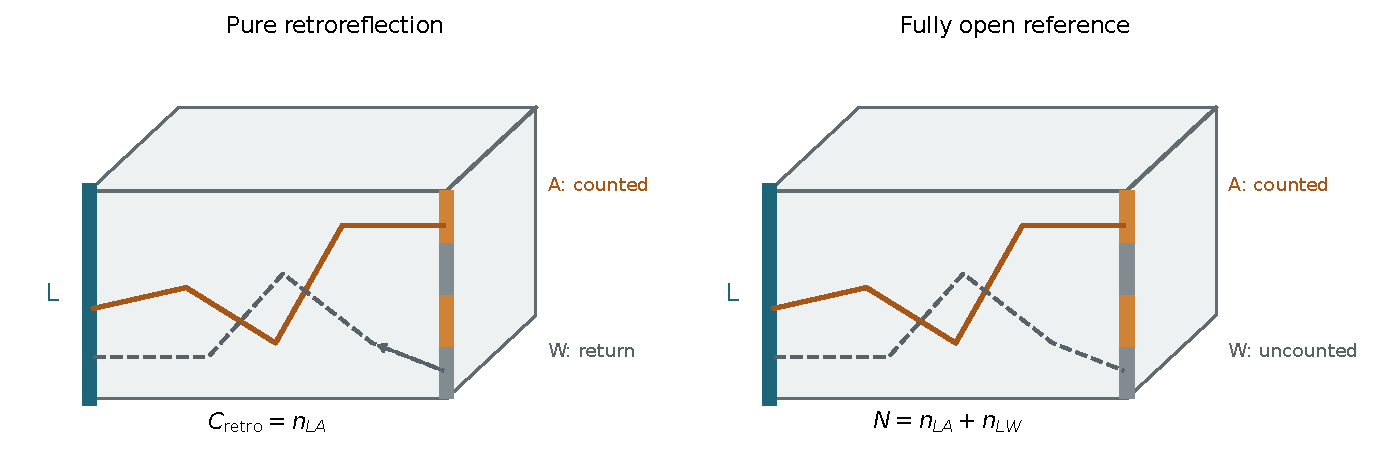
\includegraphics[width=.92\textwidth]{figures/geometry.pdf}
\caption{Opening the retroreflecting complement \(W\) converts retraced
returns to left-to-\(W\) connections. Paths counted from the full left face
to \(A\) are unchanged. The bulk environment is fixed.}
\end{figure}

\section{Conditional diffusive description}
\subsection{Finite source and inherited counting theory}
The local link-spin weight
\[
W_r=|P_r|^{-1}\sum_{P\in P_r}\prod_{(a,b)\in P}S_a\cdot S_b,\qquad
\int d\mu(S)S^aS^b=\delta_{ab}
\]
contracts to a factor \(n\) per closed loop and a boundary scalar product
per open path. Evaluating the finite polynomial at \(n=1\) recovers the mirror
ensemble. Using bilinear complex products, take
\[
u_L=(1,a,ia),\quad u_A=(1,b,-ib),\quad u_W=(1,0,0),\quad z=1+2ab.
\]
Only \(u_L\cdot u_A=z\) differs from one, yielding \(\E z^C\).
Finite enumeration and independent tensor contraction check this identity.
They do not establish the infinite-volume field theory.

Assume an ordered smooth sector, its leading isotropic gradient action and
the prescribed boundary data. Near zero source its stationary action matches
diffusive conductor counting theory \cite{NB} under
\begin{equation}
q=(1+z)/2,\quad
F_C(s)=F_e\!\left(\log\frac{1+e^s}{2}\right),\quad
v_C=(1+v_e)/2,\quad h_C=(3v_e+h_e)/4 ,
\label{eq:dictionary}
\end{equation}
with conductor mean twice the mirror mean. This is a formal generating-function
relation within the saddle. It does not identify microscopic probability
measures, fluctuation determinants, topological sectors or physical trajectories.

\subsection{Boundary functional}
Let \(\phi_L,\phi_A\) be harmonic characteristic potentials, one on their
own terminal and zero on the other open terminals, in the fully open reference.
Define
\begin{equation}
M=-\int_\Omega\nabla\phi_L\cdot\nabla\phi_A,\qquad
J=\int_\Omega|\nabla(\phi_L\phi_A)|^2 .
\end{equation}
The characteristic-potential noise integral \cite{SL} and
Eq.~\eqref{eq:dictionary} give
\begin{equation}
\log\E e^{sC}\simeq KM(e^s-1)-\frac{KJ}{2}(e^s-1)^2+\cdots,\qquad
v=1-J/M .
\label{eq:variance}
\end{equation}
The stiffness \(K\) cancels. This general structure is inherited from prior
theory; the Supplement gives the boundary-matrix comparison.

For separated right terminals with potentials \(\phi,\psi\), define \(M,J\)
in the same way. The mixed-twist coefficient predicts
\(\Cov(X,Y)/\E n_{R_1R_2}=2J/M\), where
\(X=n_{LR_1}+n_{R_1R_2}\), \(Y=n_{LR_2}+n_{R_1R_2}\).
Neumann conditions on a side-pairing wall are an additional microscopic
assumption. These tests are distinct from the exact retroreflection reduction.

\subsection{Stripe closed expression}
For a unit cube \(\phi_L=1-x\), \(M=p\), and integration by parts gives
\(J=\int\phi_A^2\). For mask Fourier coefficients \(f_n\),
\begin{equation}
J=\frac{p^2}{3}+\sum_{n\ne0}|f_n|^2I(2\pi|n|),\qquad
I(k)=\int_0^1\frac{\sinh^2(kx)}{\sinh^2k}\,dx
=\frac{\coth k}{2k}-\frac1{2\sinh^2k}.
\label{eq:fourier}
\end{equation}
For \(m\) stripes, nonzero frequencies are \(mj\), with squared coefficients
\(\sin^2(\pi jp)/(\pi j)^2\). Separating \(I(k)=1/(2k)+O(e^{-2k})\) gives,
for fixed \(0<p\leq1\),
\begin{equation}
v(p,m)=1-\frac p3-
\frac{\zeta(3)-\Re\Li_3(e^{2\pi ip})}{4\pi^3mp}+O(e^{-4\pi m}).
\label{eq:closed}
\end{equation}
At \(p=1/2\), the leading expression is
\(5/6-7\zeta(3)/(8\pi^3m)\). Numerical targets retain the exponential
correction: about \(2.60\times10^{-6}\) for \(m=1\), and below \(10^{-11}\)
for \(m=2\). The full face gives \(2/3\) exactly; the \(m\to\infty\) limit
at fixed \(p\) is \(1-p/3\). The latter matches independent binomial thinning
of a count with ratio \(2/3\), but does not establish thinning for a fixed mask.

\section{Numerical design}
The initial study used \(L=16,32,64,96\), both rules and several domain and
wall geometries. All 30 planned tests and sample allocations are in the
Supplement. The subsequent layout data set contains 2,522,250 environments
at \(L=16,32,64,128\), with paired primary contrast \(v_4-v_1\).
The fresh absolute-ratio data set contains 1,146,500 environments at
\(L=32,64,128,256\). Old and pilot samples do not enter that primary analysis.

Rules, sample counts and seeds were fixed and hashed before the respective
confirmation samples. These were \emph{local} preregistrations, without a
third-party timestamp or registry. Public hashes verify file contents,
not independently when the rules were fixed.

Both \(a+b/L\) and \(a+b/L+c/L^2\) are retained for every analysis.
These are prescribed fitting assumptions, not a derived expansion with
bounded remainder. Joint fits share only the intercept; each rule has its
own correction coefficients. Bootstrap resampling uses independent
environments, preserves paired correlations and keeps the original fixed
bootstrap seeds. No sample or size is removed because of its result.

For a half-open mask, let \(Q_m\) average \((C_m-N/2)^2\) over all transverse
translations and both orientations within an environment. Symmetry gives
\begin{equation}
\Var(C_m)=\tfrac14\Var(N)+\E Q_m,\qquad
\widehat v_m=(\tfrac12s_N^2+2\overline Q_m)/\overline N .
\end{equation}
Translated masks are not independent observations. Direct cyclic-window
sums checked the Fourier implementation on every saved environment.
The absolute-ratio analysis uses six Holm tests at level \(0.05\),
fit probabilities at least \(0.01\), rule differences within three
combined standard errors, and joint errors at most \(0.003\).
Consistency under these checks is not an equivalence proof.

\section{Results}
\subsection{Half-open stripes}
\begin{table}[htbp]\centering\small\caption{Half-open stripe ratios. Errors are bootstrap standard errors; both prescribed extrapolations use all four sizes.}
\begin{tabular}{lrrr}\toprule
$m$ & Theory & Linear & Quadratic\\\midrule
1 & 0.799413778 & $0.799752\pm0.001116$ & $0.797022\pm0.002399$\\
2 & 0.816372255 & $0.817086\pm0.001130$ & $0.812874\pm0.002408$\\
4 & 0.824852794 & $0.825861\pm0.001150$ & $0.820215\pm0.002456$\\
\bottomrule\end{tabular}\end{table}

\begin{figure}[htbp]\centering
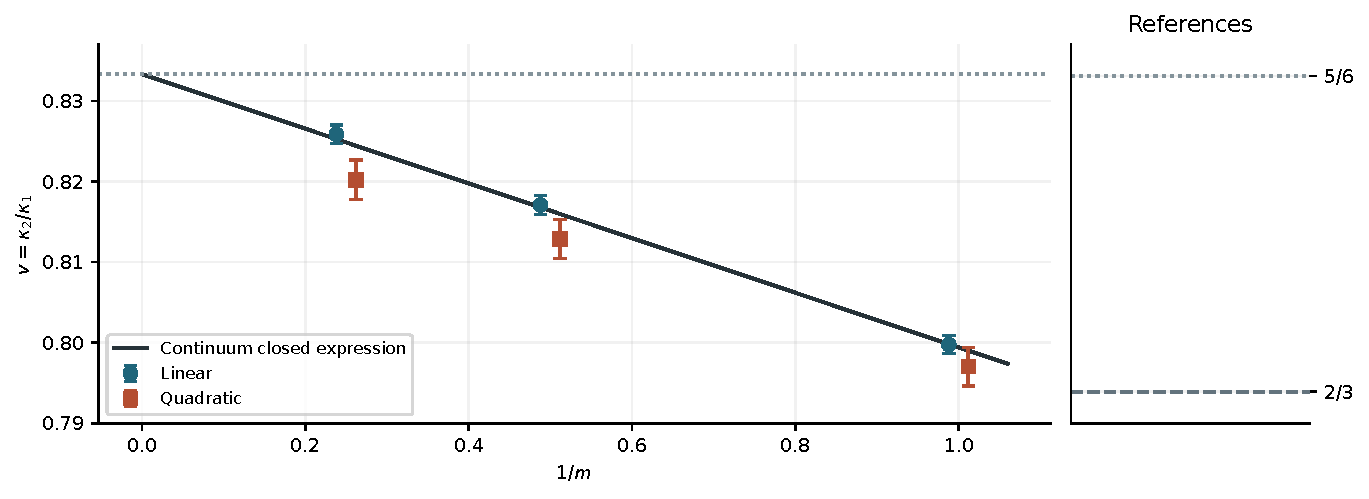
\includegraphics[width=.89\textwidth]{figures/stripe_law.pdf}
\caption{Half-open ratios versus inverse stripe number, with one-standard-error
bootstrap bars. The line omits the exponential term; tabulated targets retain
it. Horizontal offsets distinguish the two extrapolations. The right panel
uses a wider vertical range to show both limiting reference values.}
\end{figure}
All three targets lie between the joint linear and quadratic estimates.
The linear deviations are about \(0.3,0.6,0.9\) standard errors upward;
the quadratic deviations are about \(1.0,1.5,1.9\) downward.
All prescribed checks pass. The differences between forms are approximately
\(0.0027,0.0042,0.0056\), exceeding the linear statistical errors.
This spread describes extrapolation sensitivity; it is not a confidence
interval or a complete systematic-error bound.

The independent layout data reject zero difference between four and one
stripes under the original rules. Joint estimates are
\(0.02671905\pm0.00210647\) and \(0.02514860\pm0.00532498\), versus
the predicted \(0.0254390161\). This supports shape dependence without
establishing every absolute coefficient or arbitrary boundary geometry.
\begin{figure}[htbp]\centering
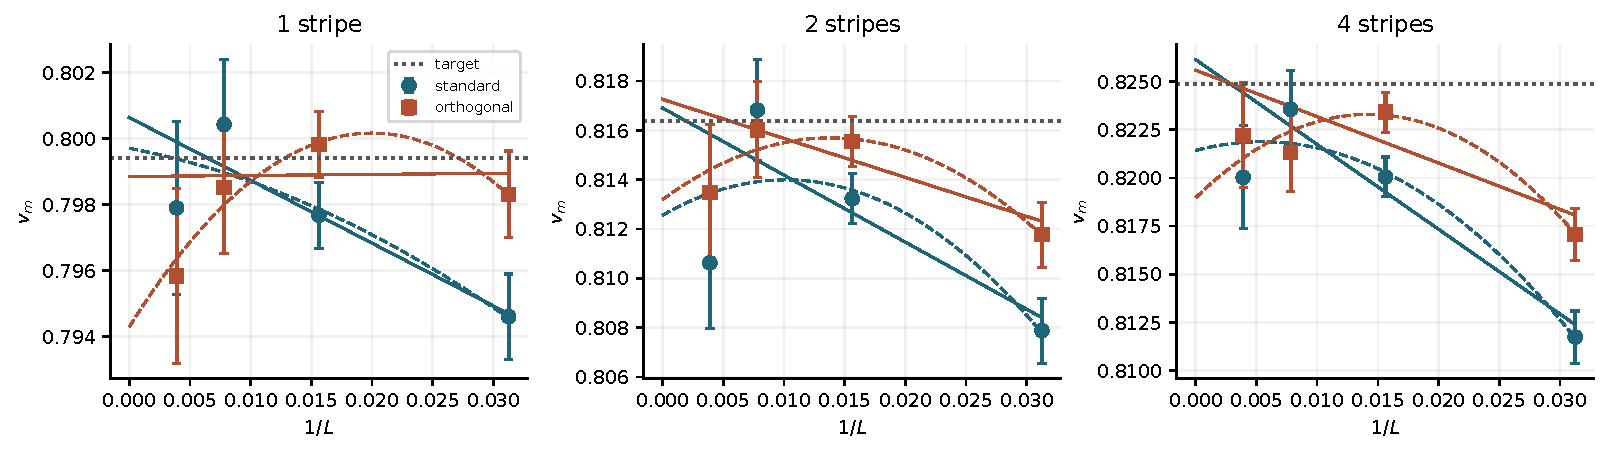
\includegraphics[width=\textwidth]{figures/finite_size.pdf}
\caption{All fresh half-open data, both rules and both prescribed separate-rule
fits (solid: linear; dashed: quadratic). No small-size points are discarded.}
\end{figure}

\subsection{Other boundaries}
\begin{table}[htbp]\centering\small\caption{Original boundary tests, with one-standard-error uncertainties. Cube and retroreflection were tested against $2/3$. The covariance target for each gapped wall is $0.5138587$ with a deterministic allowance $0.0018720$, distinct from a statistical error.}
\begin{tabular}{llrr}\toprule
Geometry / observable & Rule & Linear & Quadratic\\\midrule
Cube & Standard & $0.670186\pm0.002851$ & $0.666812\pm0.007241$\\
Cube & Orthogonal & $0.669290\pm0.003060$ & $0.669803\pm0.006917$\\
Gap, wall A & Standard & $0.517004\pm0.001513$ & $0.514276\pm0.003236$\\
Gap, wall A & Orthogonal & $0.514532\pm0.001441$ & $0.514961\pm0.003056$\\
Gap, wall B & Standard & $0.517263\pm0.001422$ & $0.517552\pm0.003278$\\
Gap, wall B & Orthogonal & $0.517928\pm0.001388$ & $0.517246\pm0.002997$\\
Retroreflection & Standard & $0.822143\pm0.002181$ & $0.822773\pm0.004819$\\
Retroreflection & Orthogonal & $0.818848\pm0.002116$ & $0.813176\pm0.004597$\\
\bottomrule\end{tabular}\end{table}

\begin{figure}[htbp]\centering
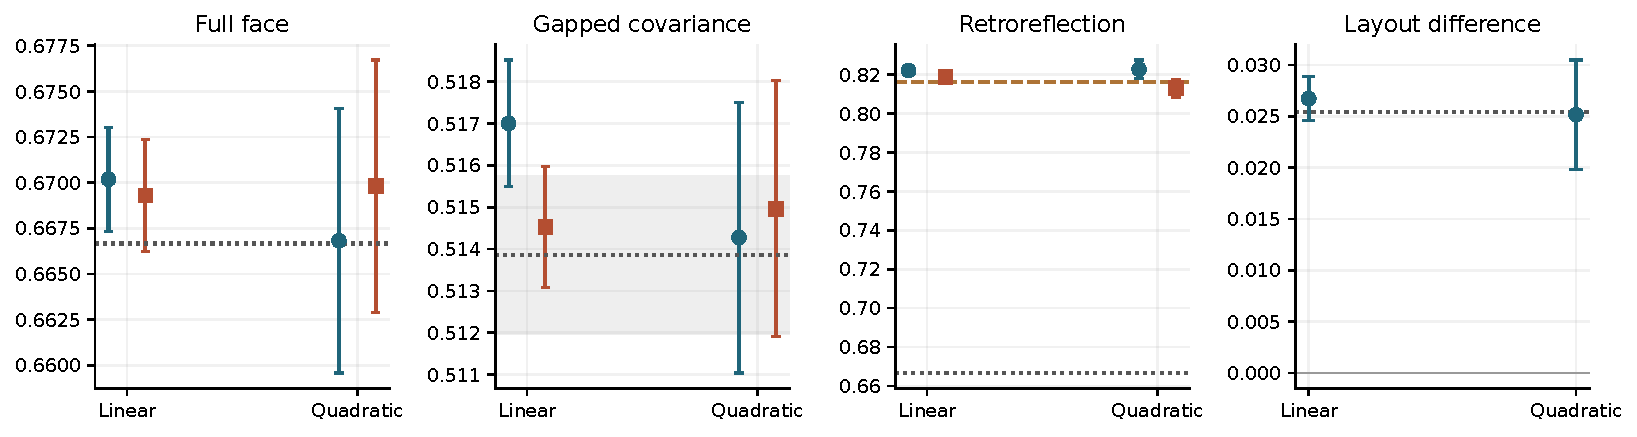
\includegraphics[width=\textwidth]{figures/other_checks.pdf}
\caption{Selected original boundary tests and the independent layout contrast.
Bars are one standard error. The covariance band is the separate deterministic
theory allowance. Teal circles denote the standard rule and rust squares
the orthogonal rule; the layout contrast uses joint fits. Retroreflection
is shown against both its original \(2/3\)
null and the later partial-port prediction (dashed).}
\end{figure}
The fully open cube is consistent with \(2/3\); separated-terminal covariance
is consistent with its conditional target for both wall wirings.
Five of the twelve related covariance-identity tests remain undecided.
The constricted-domain second-cumulant fit and one wall's third-cumulant fit
fail their adequacy checks. Fourth-cumulant tests remain inconclusive.

The original retroreflecting count robustly rejects \(2/3\).
Its later exploratory comparison to the two-stripe prediction gives
deviations between approximately \(-0.70\) and \(2.65\) standard errors.
Reconstructing \(N=C+f_L\) from the same data gives full-face intercepts
between \(0.66650\) and \(0.67085\). These are retrospective comparisons,
not new independent samples.

\subsection{Residual discrepancies}
The older standard-rule layout data have a shared linear-intercept excess
\(0.007056\pm0.001616\). Pooling both batches and all sizes leaves a
one-stripe linear excess of about \(3.4\)--\(3.5\) standard errors under
two pooling conventions, while quadratic estimates remain near theory.
Small-size curvature is a possible retrospective explanation, not an
established microscopic correction.

\begin{table}[htbp]\centering\small\caption{Exploratory quarter-open results. Joint fits are descriptive; neither batch nor rule is discarded.}
\begin{tabular}{lrrr}\toprule
Observable & Target & Linear & Quadratic\\\midrule
Quarter strip & 0.874266572 & $0.878925\pm0.001518$ & $0.878854\pm0.002585$\\
Square & 0.872115450 & $0.876012\pm0.001484$ & $0.876146\pm0.002530$\\
Square minus strip & -0.002151122 & $-0.002922\pm0.000709$ & $-0.002746\pm0.001201$\\
\bottomrule\end{tabular}\end{table}

The quarter-open layouts use 196,000 diagnostic environments including
\(L=16\), and are exploratory. Their difference is consistent with the
geometric prediction, but both absolute values are about \(0.5\%\) high.
The strip's linear estimate is about \(3.07\) standard errors above theory.
Neither form, rule nor layout is omitted.

The one-stripe third-cumulant target is \(0.4994424165\) within the saddle.
Fresh half-open data give \(0.4735764\pm0.0101997\) linearly and
\(0.4797957\pm0.0305811\) quadratically; independent diagnostic data give
\(0.5150117\pm0.0176500\) and \(0.5059868\pm0.0380576\).
The linear estimates lie on opposite sides and differ by about two
combined standard errors; the size ranges differ.
Within each batch, all three masks share the environments and the full-face
third-cumulant term, so they are not three independent pieces of evidence.
These auxiliary results supply no new confirmation decision.

\section{Limitations and open questions}
The graph reduction is exact independently of continuum theory.
The stripe predictions additionally assume a smooth diffusive phase and
appropriate boundary data. Existing transport and loop results, and the
present tests, do not prove those assumptions for the two microscopic rules.
The formal counting dictionary does not identify quantum time statistics
with quenched sample statistics.

There is no controlled remainder bounding all omitted bulk, surface,
contact-line and corner terms. Exploratory matching included microscopic
fourth- and sixth-order sources and specified one- and two-loop contributions.
It did not produce a complete physical error budget or explain the older
third-cumulant downward discrepancy. The Supplement records the scope and
failures of that attempt. Those corrections are not applied to the primary
results or their error bars.

Quarter-open absolute ratios need independent confirmation before supporting
a broader claim about \(p\ne1/2\). Their deviations do not establish failure
of the smooth description or justify neglecting finite sizes.
Higher cumulants, unresolved covariance identities and finite-precision
controls remain open. So do a rigorous long-distance limit, defect control,
and interchange of replica continuation, source differentiation and volume
limits. This is an exact boundary reduction with conditional tested
predictions, not a completed microscopic field theory.

\section*{Data, code and contributions}
The \href{https://github.com/SHIN09-git/mirror3d-partial-ports/releases/tag/v1.0.0}{versioned release} includes compact observations for every
environment in both stripe data sets, original seeds and local registration
files, summaries and reproduction scripts. Full original blocks and historical
failed runs remain separately preserved. Compact records support the primary
analyses, not every auxiliary higher-order response.

JJIN HANZHE provided directional guidance. Opus 5.5 proposed the initial plan;
GPT-6 Astra (max) performed later design, simulations, analysis, derivations
and writing. Checks use separate implementations, exact identities and
independent numerical calculations, not agreement between AI systems.
There has been no external human expert review.
Code is licensed MIT; manuscript and data are licensed CC BY 4.0.

\appendix
\section{Fourier identity and omitted term}
The harmonic profile \(\sinh(kx)/\sinh k\) directly integrates to
Eq.~\eqref{eq:fourier}. The zero mode \(px\) contributes \(p^2/3\).
With \(r=e^{-2k}\),
\[
I(k)-\frac1{2k}=\frac{r}{k(1-r)}-\frac{2r}{(1-r)^2},\qquad
\sum_{j\ge1}\frac{\sin^2(\pi jp)}{j^3}
=\frac{\zeta(3)-\Re\Li_3(e^{2\pi ip})}{2}.
\]
For rational \(p\), an independent Hurwitz-zeta residue-class sum and
numerical kernel integration reproduce the targets. The square window
requires a two-dimensional sum with an explicit positive tail bound.
Neither numerical bound controls microscopic finite-size effects.
\bibliographystyle{unsrt}
\bibliography{refs}
\end{document}
